
\ابتدا{مثال}
شکل \حوالہ{شکل_امالہ_مروڑ_مستطیل} میں مستطیل دکھایا گیا ہے جس میں \عددی{\SI{2}{\ampere}} کی برقی رو گردش کر رہی ہے۔محدد \عددی{z} میں \عددی{\az} جانب \عددی{\SI{1.5}{\ampere}} کی برقی رو گزر رہی ہے۔محدد کے مرکز کو محور تصور کرتے ہوئے مستطیل پر مروڑ دریافت کریں۔
\begin{figure}
\centering
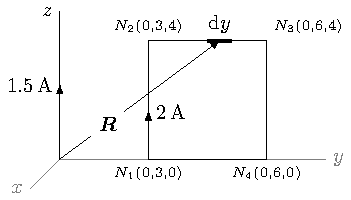
\includegraphics{figInductanceTorqueOnRectangularLoop}
\caption{مستطیل پر مروڑ کا حساب۔}
\label{شکل_امالہ_مروڑ_مستطیل}
\end{figure}

حل:محدد \عددی{z} پر برقی رو
\begin{align*}
\kvec{B}&=\frac{1.5 \mu_0}{2\pi \rho}\aphi
\end{align*}
میدان پیدا کرے گی جسے مستطیل کے احاطے میں
\begin{align*}
\kvec{B}=-\frac{1.5\mu_0}{2\pi y}\ax
\end{align*}
لکھا جا سکتا ہے۔یہ میدان \عددی{y} کے تبدیلی سے تبدیل ہوتا ہے لہٰذا یہ غیر یکساں میدان ہے۔غیر یکساں میدان میں مروڑ کا دارومدار محور پر ہوتا ہے لہٰذا ہمیں محدد کے مرکز \عددی{(0,0,0)} کو ہی محور لینا ہو گا۔آئیں \عددی{N_2} اور \عددی{N_3} کے مابین تار پر مروڑ حاصل کریں۔چھوٹی لمبائی \عددی{\dif y} پر تفرقی قوت 
\begin{align*}
\dif \kvec{F}_{32}&=2 \dif y \ay \times \left(-\frac{1.5\mu_0}{2\pi y}\ax \right)
\end{align*} 
\انتہا{مثال}
